\documentclass{standalone}

\usepackage{tikz}
\usepackage{bm}

\usetikzlibrary{patterns}
\usetikzlibrary{arrows.meta}

\usetikzlibrary{decorations.pathreplacing, decorations.markings}
\tikzset{
    midarrow/.style={
        decoration={markings, mark=at position 0.5 with {\arrow{Latex}}},
        postaction={decorate}
    }
}

\usetikzlibrary{spy}

\begin{document}

\begin{tikzpicture}[spy using overlays={size=20mm}]
	\pgfmathsetmacro{\x}{0}
	
	\foreach \i in {0, ..., 10} {
			\pgfmathsetmacro{\x}{\i/3+(rand-0.5)/10-1}
			\draw[ midarrow ] (\x,0) arc[start angle=90, end angle=-90, radius=1];
	}
	
	\foreach \i in {10, 8, 6, 4, 2, 0} {
			\pgfmathsetmacro{\x}{\i/3+rand/10}
			\draw[ midarrow ] (\x,-2) arc[start angle=270, end angle=90, radius=1];
	}
	
	\spy [black!70, magnification=2] on (10/6-0.5, -1) in node at (10/3+2,-1);
	
\end{tikzpicture}

\end{document}